\fancyhead[RO,LE]{\thepage}
\fancyfoot{} 
\chapter{Technical Background and Related Work}
\label{chapter:background}

In this chapter I describe the technical background and related work most relevant to my research. I begin this chapter  by discussing an emerging research field that seeks to accelerate general-purpose computations by performing them on GPUs. I motivate the use of GPUs for general-purpose computation with a discussion of their performance advantages. I introduce the \emph{stream programming model} -- an abstract programming model used to design massively parallel algorithms suitable for execution on the GPU. I introduce a set of mathematical tools used to analyze the asymptotic performance of algorithms expressed in the stream programming model. I also discuss two fundamental stream operations that are required in my research. The first operation is known as \emph{all-prefix-sums} (sometimes referred to as \emph{scan}) and involves computing the sum of all elements prior to each element in an input array. The second operation is known as \emph{stream compaction} and involves removing unwanted elements from an input array. I show that stream compaction can be trivially  implemented in terms of all-prefix-sums. I conclude this chapter by describing the current state-of-the-art algorithms for GPU level set segmentation, as well as a CPU level set segmentation algorithm that influenced my research.

%*******************************************************************************
% FIGURE Technology Trends
\begin{figure}[t]
\centering
\subfigure[]{
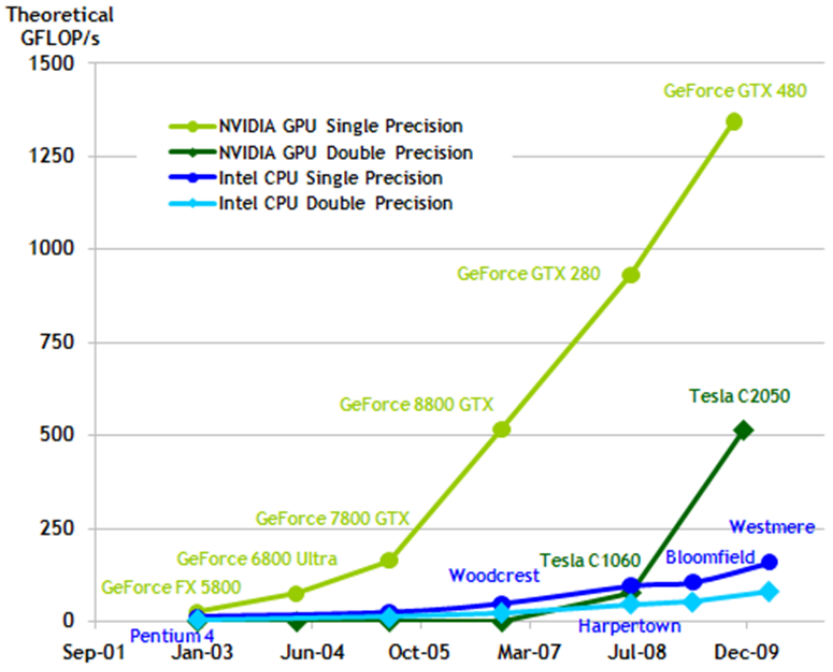
\includegraphics[width=4.0in]{figures/gflops.png}
}
\subfigure[]{
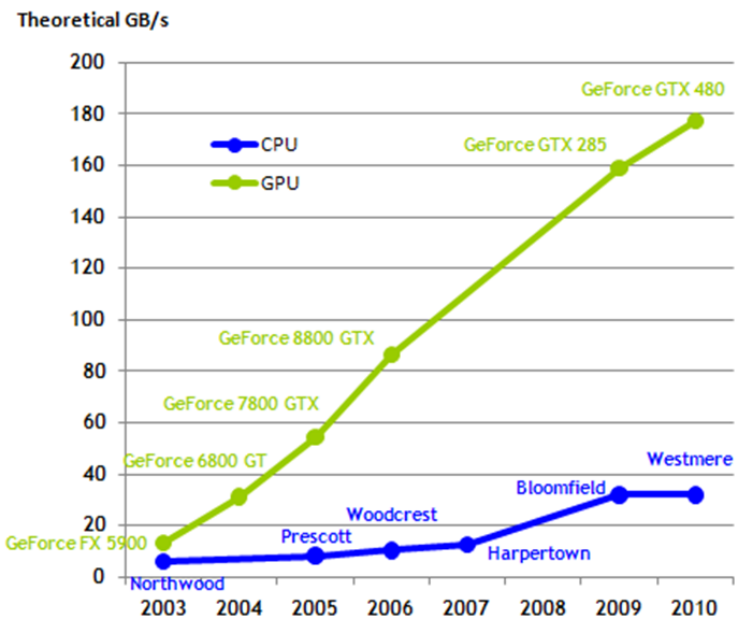
\includegraphics[width=4.0in]{figures/bandwidth.png}
}
\caption{Performance trends for GPUs and CPUs as indicated by floating-point operations per second (GFLOPS) (a) and memory bandwidth (GB/sec) (b)~\cite{NVIDIACUDA-2010}.}
\label{fig:gpu-cpu-performance}
\end{figure}
%*******************************************************************************

\section{General-Purpose Computation on GPUs}

\subsection{GPUs are Powerful, Inexpensive, and Massively Parallel}
In the most comprehensive survey to date relating to general-purpose computation on the GPU~\cite{Owens-2007} -- an emerging research field known as \emph{GPGPU} -- Owens et al.\ write that "GPUs are probably the most powerful computational hardware for the dollar"~\cite{Owens-2007}. Owens et al.\ argue,
\begin{quote}
"graphics architectures provide tremendous provide tremendous memory bandwidth and computational horsepower. For example, the flagship NVIDIA GeForce 7900 GTX (\$378 as of October 2006) boasts 51.2 GB/sec memory bandwidth; the similarly priced ATI Radeon X1900 XTX can sustain a measured 240 GFLOPs, both measured with GPUBench~\cite{Buck-2004}. Compare to 8.5 GB/sec and 25.6 GFLOPS theoretical peak for the SSE units of a dual-core 3.7 GHz Intel Pentium Extreme Edition 965~\cite{Intel-2006}."~\cite{Owens-2007}
\end{quote}

Owens et al.\ go on to argue,
\begin{quote}
"graphics hardware is fast and getting faster quickly. For example, arithmetic throughput (again measured by GPUBench) of NVIDIA's current-generation launch product, the GeForce 7800 GTX (165 GFLOPS), more than triples that of its predecessor, the GeForce 6800 Ultra (53 GFLOPS). In general the computational capabilities of GPUs, measured by the traditional metrics of graphics performance, have compounded at an average yearly rate of 1.7 (pixels/second) to 2.3 (vertices/second). This rate of growth significantly outpaces the often-quoted Moore's Law as applied to traditional microprocessors; compare to a yearly rate of roughly 1.4 for CPU performance~\cite{Ekman-2005}."~\cite{Owens-2007}  
\end{quote}

The technology trends Owens et al.\ discuss are shown in Figure \ref{fig:gpu-cpu-performance}.

In addressing the question of why GPU performance increases faster than CPU performance, Owens et al.\ write,
\begin{quote}
"semiconductor capability, driven by advances in fabrication technology, increases at the same rate for both [CPU and GPU] platforms. The disparity can be attributed to fundamental architectural differences: CPUs are optimized for high performance on sequential code, with many transistors dedicated to extracting instruction-level parallelism with techniques such as branch prediction and out-of-order execution. On the other hand, the highly data-parallel nature of graphics computations enables GPUs to use additional transistors more directly for computation, achieving higher [computational throughput] with the same transistor count."~\cite{Owens-2007}
\end{quote}

GPUs take advantage of the abundant data parallelism in computer graphics by concurrently processing data elements on a large number of parallel cores. For example NVIDIA's current flagship GPU in August 2010, the NVIDIA GeForce GTX 480, contains 512 parallel computational cores~\cite{NVIDIAGeForceGTX480-2010}. Moreover the number of parallel computational cores on NVIDIA\ GPUs has roughly doubled every year for the last three years~\cite{NVIDIAGeForce9800-2010,NVIDIAGeForceGTX280-2010,NVIDIAGeForceGTX480-2010}. This trend is likely to continue for at least the next decade. This is because the number of transistors per die on GPUs is likely to double each year for at least the next decade~\cite{Owens-2005}, and for much longer there will likely be enough data parallelism in computer graphics to increase effective performance by adding computational cores. From the arguments above, we see that the GPU is a powerful, inexpensive, and massively parallel processor.

\subsection{Writing General-Purpose GPU Programs Using the Stream Programming Model}

Until very recently the computational power of the GPU was only available  through graphics APIs like OpenGL, DirectX, and their corresponding languages for describing geometric and optical properties of surfaces -- known as \emph{shading languages}. In order to solve non-graphics problems using GPUs, programmers were historically required to cast the computations in terms of graphics primitives. Of this programming model, Owens et al.\ write, 
\begin{quote}
"more often than not, the graphics-centric nature of shading languages makes GPGPU programming more difficult than it needs to be. As a simple example, initiating a GPGPU computation usually involves drawing a primitive. Looking up data from memory is done by issuing a texture fetch. The GPGPU program may conceptually have nothing to do with drawing geometric primitives and fetching textures, yet the shading languages described in the previous section force the GPGPU application writer to think in terms of geometric primitives [...] and textures. Instead, GPGPU algorithms are often best described as memory and math operations, concepts much more familiar to CPU programmers."~\cite{Owens-2005}
\end{quote}

Fortunately it is now possible to write general purpose programs that execute in parallel on the GPU without needing to awkwardly cast the computations in terms of graphics primitives. Instead, new GPU programming languages allow data parallel algorithms to be expressed in the more abstract \emph{stream programming model}. This programming model inherently structures algorithms in a way that expresses abundant data parallelism and transparently scales performance with the number of available parallel computational cores. The stream programming model is well suited to express data parallel algorithms in a way that can be efficiently mapped to massively parallel GPU hardware.

Owens describes the stream programming model,
\begin{quote}
"In the stream programming model, all data is represented as a \emph{stream}, which we define as an ordered set of data of the same data type. That data type can be simple (a stream of integers or floating-point numbers) or complex (a stream of points or triangles or transformation matrices). While a stream can be any length, we will see that operations on streams are most efficient if streams are long (hundreds or more elements in a stream). Allowed operations on streams include copying them, deriving substreams from them, indexing into them with a separate index stream, and performing computation on them with \emph{kernels}.

A kernel operates on entire streams, taking one or more streams as inputs and producing one or more streams as outputs. The defining characteristic of a kernel is that it operates on entire streams  of elements as opposed to individual elements. The most typical use of a kernel is to evaluate a function on each element of an input stream; for example, a transformation kernel may project each element of a stream of points into a different coordinate system. Other desirable kernel operations include expansions (in which more than one output element is produced for each input element), reductions (in which more than one element is combined into a single output element), or filters (in which a subset of input elements are output).

Kernel outputs are functions only of their kernel inputs, and within a kernel, computations on one stream element are never dependent on computations on another element. These restrictions have two major advantages. First, the data required for kernel execution is completely known when the kernel is written (or compiled). Kernels can thus be highly efficient when their input elements and their intermediate computed data are stored locally  or are carefully controlled global references. Second, requiring independence of computation on separate stream elements within a single kernel allows mapping what appears to be a serial kernel calculation onto data-parallel hardware.

In the stream programming model, applications are constructed by chaining multiple kernels together."~\cite{Owens-2005}
\end{quote}
%*******************************************************************************
\begin{Listing}[t]
    \caption{High level parallel pseudo-code for computing the $n$-dimensional vector $R$ as the sum of the two $n$-dimensional vectors $A$ and $B$. A subscript notation is used to denote individual vector elements. For example $R_{i}$ refers to the $i^{th}$ element of $R$.}
    \begin{algorithmic}[1]
        \FORALL { $ i \gets 0 \mbox{ to } n \mbox{ \ in parallel}$ } 
            \STATE { $ R_{i} \gets A_{i} +B_{i} $ }
        \ENDFOR
    \end{algorithmic}
    \label{alg:high-level-vector-add}
\end{Listing}
%*******************************************************************************
%*******************************************************************************
\begin{Listing}[t]
    \caption{Expressing the high-level parallel pseudo code from Listing \ref{alg:high-level-vector-add} as a stream program. Note that the \textbf{VectorAdd} kernel is written as though it is only processing a single element. The computation in this kernel is implicitly mapped to all stream elements and performed in parallel on the stream processor.}
    \scriptsize
    \begin{verbatim}
// this kernel adds two N-dimensional vectors in parallel
kernel VectorAdd( stream result<>, stream int a<>, stream int b<> )
{
    result = a + b;
}

// this program adds two N-dimensional vectors together in parallel 
void main()
{
    // define int arrays in main memory
    int a[N], int b[N];
    
    // define int streams on the stream processor
    stream int sA<N>, sB<N>, sResult<N>;
 
    // ... initialize the input arrays ...
    
    // ... copy the contents of the input arrays into the input streams ...
        
    // invoke the VectorAdd kernel
    VectorAdd( sResult, sA, sB );

    // ... at this point sResult contains the results of the vector addition ...
}
    \end{verbatim}
    \label{alg:stream-program-vector-add}
\end{Listing}
%*******************************************************************************
Listing \ref{alg:high-level-vector-add} shows high level parallel pseudo-code for adding two $n$-dimensional vectors, and Listing \ref{alg:stream-program-vector-add} shows how this pseudo-code would be expressed as a stream program.

\subsection{Asymptotic Complexity}

We are often interested in analyzing the efficiency of algorithms independently from the performance characteristics of the machine on which they are executing. Rather than directly measuring number of operations an algorithm performs for a particular input, we determine the amount of work an algorithm performs, and the amount of memory it consumes, as a function of input size for arbitrarily large inputs.
We refer to this abstract measure of efficiency as an algorithm's \emph{asymptotic} complexity.

\subsection{Analyzing the Asymptotic Complexity of Stream Algorithms}

To analyze the asymptotic behavior of sequential algorithms, we assume the algorithm executes on a theoretical processor that performs one canonical unit of work per unit of time. This theoretical computational model is known as the random access machine (RAM) model, and the theoretical processor is known as a RAM processor.~\cite{Atallah-1998}

Analyzing the asymptotic behavior of parallel algorithms requires us to extend this model. Again our goal is to analyze the parallel algorithm independently from the physical system on which it is running. Therefore in our extended theoretical computational model, we assume there are an unbounded number of RAM processors and that all these processors share a common memory. This is known as the \emph{\emph{parallel random access machine}} (PRAM) model, and the parallel processors are known as PRAM processors.~\cite{Atallah-1998}

In the RAM model, the amount of work a sequential algorithm performs is equal to the amount of time it takes to execute. In the PRAM model, this is equality does not hold in general, since more than one processor may be doing a unit of work in a unit of time. Therefore determining the asymptotic runtime complexity of parallel algorithms involves deriving expressions for two important quantities. The first quantity is known as \emph{work-complexity}, which refers to the total amount of work performed by the parallel algorithm~\cite{Atallah-1998}. The second quantity is known as \emph{step-complexity}, which refers to the total number of steps (i.e. units of time) required for the parallel algorithm to execute, given the unbounded number of processors in the PRAM model~\cite{Nyland-2000}.

A parallel algorithm is \emph{work-efficient} if it performs asymptotically no more work than the most efficient sequential algorithm. In practice it is important for parallel algorithms to be work-efficient. If a parallel algorithm is not work-efficient, and it is executed on a machine with a finite number of processors, then the most efficient sequential algorithm will outperform the parallel algorithm on sufficiently large inputs.~\cite{Atallah-1998}

A parallel algorithm is \emph{step-efficient} if it requires asymptotically fewer steps to execute than the most efficient sequential algorithm. It is important for parallel algorithms to be step-efficient. If a parallel algorithm is not step-efficient, there is no asymptotic benefit to using the parallel algorithm over the most efficient sequential algorithm.

\phantomsection
\subsection{All-Prefix-Sums}
\phantomsection

The \emph{all-prefix-sums} operation, also known as \emph{scan}, is one of the most important primitive operations for constructing data parallel algorithms. All-prefix-sums involves computing, for every element of an input array, the sum of all the previous elements in the array. All-prefix-sums can be used to implement efficient parallel algorithms for quick-sort, radix-sort, sparse matrix multiplication, removing marked elements from arrays, parsing strings into tokens, lexicographic sorting, constructing data structures for fast image filtering, and many other fundamental tasks~\cite{Blelloch-1993,Hensley-2005}. In particular, all-prefix-sums is an important primitive operation in the parallel level set segmentation algorithm described in Chapter \ref{chapter:parallel}, since this algorithm requires an efficient parallel method for removing marked elements from arrays.

\begin{samepage}
For the purposes of this thesis, I define all-prefix-sums as follows:
\begin{quote}
Given the following input array of size $n$,
\end{quote}
\begin{equation}
\left[ a_0 , a_1 , a_2 , \ldots , a_n \right]
\end{equation}
\begin{quote}
all-prefix-sums returns the following array as output,
\end{quote}
\begin{equation}
\left[0,a_0,\left(\sum_{ i = 0 }^{ 1 } a_i\right),\left(\sum_{ i = 0 }^{ 2 } a_i\right),\left(\sum_{ i = 0 }^{ 3 } a_i\right),\ldots,\left(\sum_{ i = 0 }^{ n-1 } a_i\right)\right]
\end{equation}
\begin{quote}
For example, if the input array was $[10, 4, 6, 8, 4, 3, 2, 5]$, the output of all-prefix-sums would be the array $[0,10,14,20,28,32,35,37]$.
\end{quote}
\end{samepage}

%*******************************************************************************
\begin{Listing}[t]
    \caption{Sequential pseudo-code for computing all-prefix-sums of an input array $A$ and storing the results in an output array $R$. A subscript notation is used to denote individual array elements. For example $R_{i}$ refers to the $i^{th}$ element of $R$. }
    \begin{algorithmic}[1]
        \STATE { $ R_0 \gets 0 $ }
        \FOR { $ i \gets 1 \mbox{ to } n $ } 
            \STATE { $ R_{i} \gets R_{ i - 1 } + A_{i} $ }
        \ENDFOR
    \end{algorithmic}
    \label{alg:sequential-all-prefix-sums}
\end{Listing}
%*******************************************************************************

A trivial sequential algorithm for all-prefix-sums is shown in Listing \ref{alg:sequential-all-prefix-sums}. I note that this algorithm performs $O(n)$ work. This algorithm cannot be parallelized straight-forwardly since each iteration of the \textbf{for} loop in Listing \ref{alg:sequential-all-prefix-sums} depends on the previous iteration. Sengupta et al.\ discuss the challenges involved in parallelizing all-prefix-sums,

\begin{quotation}
"How do we compute the value of the last element in the output? That value is a function of \emph{every} value in the input stream. With a serial processor, such a computation is trivial, but with a parallel processor, it is more difficult. The naive way to compute each output in parallel is for every element in the output stream to sum all preceding values from the input stream. This approach requires $O(n^2)$ total memory accesses and addition operations. This cost is too high."~\cite{Sengupta-2007}
\end{quotation}

Blelloch introduced a work-efficient and step-efficient parallel algorithm for all-prefix-sums that avoids the costs of the naive algorithm~\cite{Blelloch-1993}. He also discussed all-prefix-sums in the context of several important data parallel applications~\cite{Blelloch-1993}. Horn introduced the first GPU algorithm for all-prefix-sums as part of a collision-detection application~\cite{Horn-2005}. Hensley et al.\ improve on the performance of Horn's GPU implementation in their work on fast image filtering~\cite{Hensley-2005}. Although these GPU algorithms are step-efficient, they are not work-efficient. This inefficiency has a significant impact on practical performance, especially for large arrays. Sengupta et al.\ and Gre\ss \ et al.\ each describe work-efficient GPU algorithms for all-prefix-sums~\cite{Sengupta-2006,Greb-2006}. Harris et al.~\cite{Harris-2007}, Dotsenko et al.~\cite{Dotsenko-2008}, and Sengupta et al.~\cite{Sengupta-2011} improve on the performance of these GPU algorithms and preserve their asymptotic properties.~\cite{Sengupta-2007}

Harris et al.\ provide a high-level description of the work-efficient GPU all-prefix-sums algorithm used in this thesis,
\begin{quotation}
"We would like to find an algorithm that would approach the efficiency of the sequential algorithm, while still taking advantage of the parallelism in the GPU. Our goal in this section is to develop a work-efficient scan algorithm [...] based on the one presented by Blelloch~\cite{Blelloch-1993}. To do this we will use an algorithmic pattern that arises often in parallel computing: balanced trees. The idea is to build a balanced binary tree on the input data and sweep it to and from the root to compute the prefix sum. A binary tree with $n$ leaves has $d = \log_2n$ levels, and each level $d$ has $2^d$ nodes. If we perform one add per node, then we will perform $O(n)$ adds on a single traversal of the tree."
\end{quotation}

In other words, if we perform one operation per node for a balanced binary tree with $n$ leaves, then we will have performed a total of $2n - 1$ operations. Therefore each time we sweep across the entire tree performing one operation per node, we will have performed $O(n)$ operations.
Harris et al. goes on to describe this concept of distributing work across a balanced binary tree in more detail,
\begin{quotation}
"The tree we build is not an actual data structure, but a concept we use to determine what each thread does at each step of the traversal. The algorithm consists of two phases: the up-sweep phase and the down-sweep phase. In the up-sweet phase, we traverse the tree from leaves to root computing partial sums at internal nodes of the tree, as shown in Figure \ref{fig:upsweep}. Pseudo-code for the up-sweep phase is given in Listing \ref{alg:all-prefix-sums-upsweep}.

In the down-sweep phase, we traverse back down the tree from the root, using the partial sums from the reduce phase to build the scan in place on the array. We start by inserting zero at the root of the tree, and on each step, each node at the current level passes its own value to its left child, and the sum of its value and the former value of its left child to its right child. The down-sweep is shown in Figure \ref{fig:downsweep}, and pseudo-code is given in Listing \ref{alg:all-prefix-sums-downsweep}."~\cite{Harris-2007}
\end{quotation}

In principle this all-prefix-sums algorithm sweeps twice across a balanced binary tree with $n$ leaves. Therefore it performs $O(n)$ work. The operations at each level of the tree are independent, and can therefore be performed in parallel in a single step. Since there are $\log_2 n$ levels in the tree, each sweep across the tree requires $O(\log_2 n)$ steps. Therefore this all-prefix-sums algorithm is both work-efficient and step-efficient.
\pagebreak
%*******************************************************************************
% Upsweep
\begin{figure*}[t]
\centering
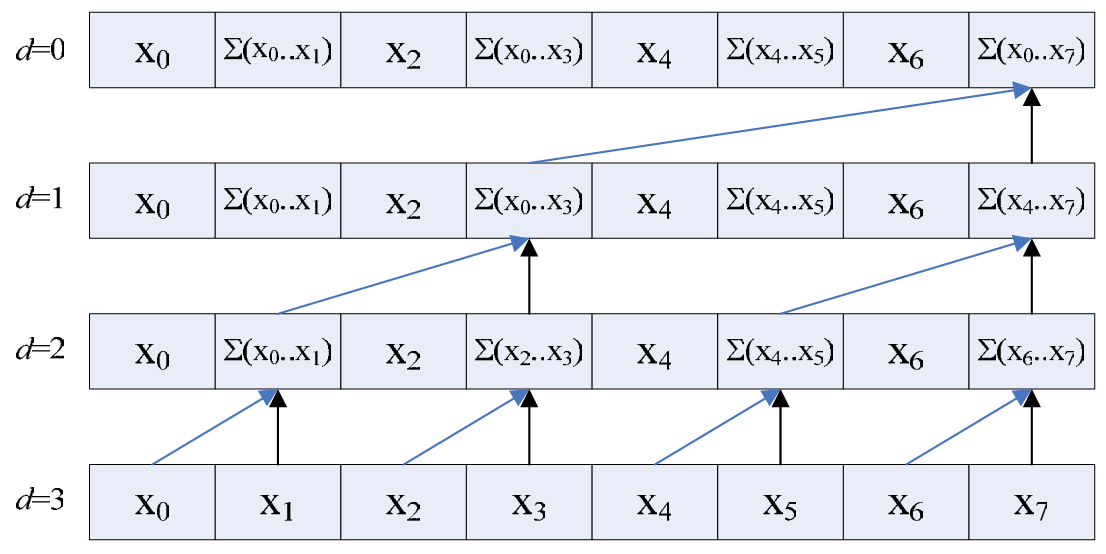
\includegraphics[width=6.0in]{figures/upsweep.png}
\caption{The up-sweep phase of the work-efficient parallel \emph{all-prefix-sums} algorithm used in this thesis~\cite{Blelloch-1993,Harris-2007,Sengupta-2011}. Each row $d$ refers to one step of the up-sweep algorithm. The bottom row ($d=3$) is the input list. The up-sweep algorithm begins at the leaf nodes ($d=3$) and proceeds up the tree to the root ($d=0$). Pseudo-code for this algorithm is given in Listing \ref{alg:all-prefix-sums-upsweep}.}
\label{fig:upsweep}
\end{figure*}
%*******************************************************************************
%*******************************************************************************
\begin{Listing}[t]
    \caption{Parallel pseudo-code for the up-sweep phase of the work-efficient parallel \emph{all-prefix-sums} algorithm used in this thesis. The input is an array $A$ of size $n$. The output is written in-place in $A$. After this up-sweep phase has completed, $A$ must undergo the down-sweep phase given in Listing \ref{alg:all-prefix-sums-downsweep}. After this down-sweep phase, $A$ will contain the final output of the all-prefix-sums operation. A subscript notation is used to denote individual array elements. For example $A_{i}$ refers to the $i^{th}$ element of $A$.~\cite{Blelloch-1993} }
    \begin{algorithmic}[1]
        \FOR { $ d \gets \log_2(n) - 1 \mbox{ down to } 0$ } 
            \STATE { $ k \gets \log_2(n) - d $ } 
            \FORALL { $ i \gets 0 \mbox{ to } n-1  \mbox{ \ incrementing by } 2^{k} \mbox{ \ in parallel } $ } 
                \STATE { $ A_{i + 2^{k}-1} \gets A_{i + 2^{k-1}-1} + A_{i + 2^{k}-1} $ }
            \ENDFOR
        \ENDFOR
    \end{algorithmic}
    \label{alg:all-prefix-sums-upsweep}
\end{Listing}
%*******************************************************************************
\clearpage
%*******************************************************************************
% Downsweep
\begin{figure*}[t]
\centering
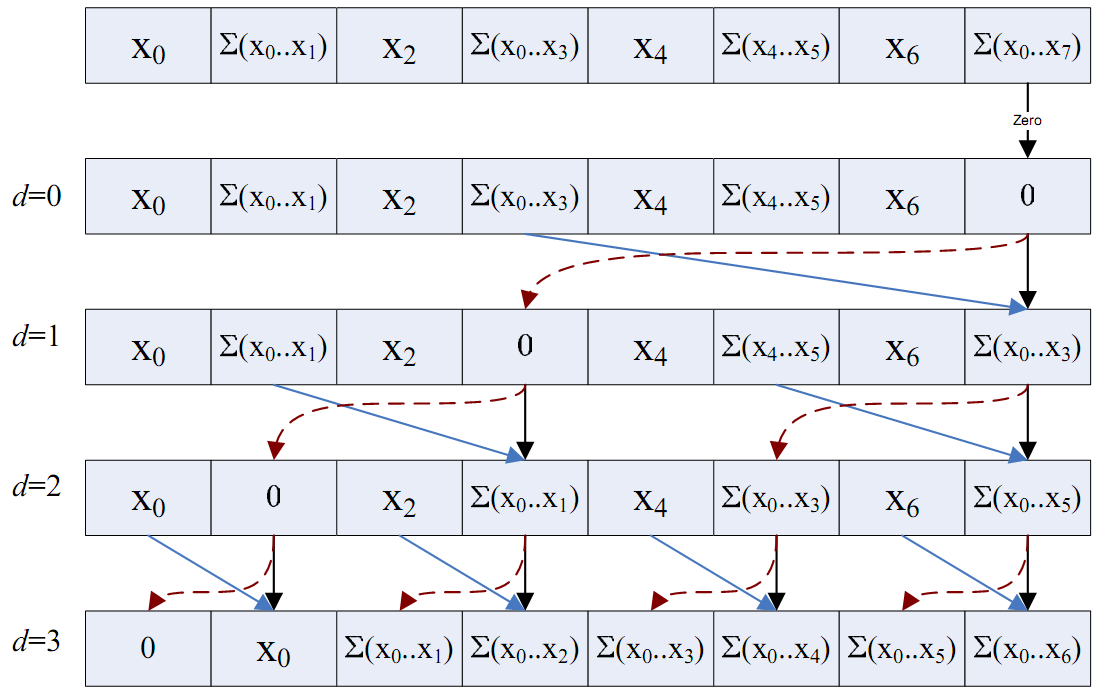
\includegraphics[width=6.0in]{figures/downsweep.png}
\caption{The down-sweep phase of the work-efficient parallel \emph{all-prefix-sums} algorithm used in this thesis~\cite{Blelloch-1993,Harris-2007,Sengupta-2011}. Each row $d$ refers to one step of the down-sweep algorithm. The top row is given by the results of the up-sweep algorithm shown in Figure \ref{fig:upsweep}. The down-sweep algorithm begins at the root node of the tree ($d=0$) and proceeds down the tree to the leaf nodes ($d=3$). Pseudo-code for this algorithm is given in Listing \ref{alg:all-prefix-sums-downsweep}}
\label{fig:downsweep}
\end{figure*}
%********************************************************************************
%********************************************************************************
\begin{Listing}[h]
    \caption{Parallel pseudo-code for the down-sweep phase of the work-efficient parallel \emph{all-prefix-sums} algorithm  used in this thesis. The input is an array $A$ of size $n$ that has undergone the up-sweep phase given in Listing \ref{alg:all-prefix-sums-upsweep}. The output is written in-place in $A$. After this algorithm has completed, $A$ will contain the final output of the \emph{all-prefix-sums} operation. A subscript notation is used to denote individual array elements. For example $A_{i}$ refers to the $i^{th}$ element of $A$.~\cite{Blelloch-1993}}
    \begin{algorithmic}[1]
        \STATE{ $ A_{n-1} \gets 0$ }
        \FOR { $ d \gets 1 \mbox{ to } \log_2(n) - 1 $ }
            \STATE{ $ k \gets \log_2(n) - d$
            \FORALL { $ i \gets 0 \mbox{ to } n - 1 \mbox{ \ incrementing by } 2^{k} \mbox{ \ in parallel } $ } 
                \STATE { $ t \gets A_{i + 2^{k-1}-1}$ }
                \STATE { $ A_{i + 2^{k-1}-1} \gets A_{i + 2^{k}-1} $ }
                \STATE { $ A_{i + 2^{k}-1} \gets t + A_{i + 2^{k}-1} $ }
            \ENDFOR
        \ENDFOR
    \end{algorithmic}
    \label{alg:all-prefix-sums-downsweep}
\end{Listing}
%********************************************************************************
\clearpage
\subsection{Stream Compaction}
Removing unwanted elements from a data stream -- an operation known as \emph{stream compaction} -- is an important task in many parallel algorithms~\cite{Blelloch-1993,Horn-2005,Ziegler-2006,Billeter-2009}, including the parallel level set segmentation algorithm described in Chapter \ref{chapter:parallel}. Given a data array and a flag array that indicates which elements should be kept from the data array, the stream compaction operation returns a dense array of all the elements from the data array that were marked for retention, with none of the elements that were marked for deletion.
\begin{samepage}
For the purposes of this thesis, I define the stream compaction operation as follows:
\begin{quote}
Given the following input data array $A$ of size $n$,
\end{quote}
\begin{equation}
\left[ a_0 , a_1 , a_2 , \ldots , a_n \right]
\end{equation}
\begin{quote}
and an input flag array $F$ of size $n$,
\end{quote}
\begin{eqnarray}
\left[ f_0 , f_1 , f_2 , \ldots , f_n \right] & \mbox{ where } & \forall_{0 \leq i \leq n} : f_i \in \{\mbox{\textbf{remove}},\mbox{\textbf{keep}}\} &
\end{eqnarray}
\begin{quote}
I define a list of size $k \leq n$,
\end{quote}
\begin{eqnarray}
[l_0,l_1,l_2,\ldots,l_k] & \mbox{ where } & \forall_{0 \leq i \leq k} : f_{l_i} = \mbox{\textbf{keep}} \\
& & \forall_{ j : f_j = \mbox{\textbf{keep}} }: \exists_{ 0 \leq i \leq k } : j=l_i \\
& & \forall_{0 \leq i,j \leq k} : {l_i} = l_j \equiv i=j \\
& & \forall_{0 \leq i,j \leq k} : {l_i} < l_j \equiv i < j
\end{eqnarray}
\begin{quote}
The stream compaction operation returns the array,
\end{quote}
\begin{equation}
\left[ a_{l_0} , a_{l_1} ,a_{l_2} , \ldots , a_{l_k} \right]
\end{equation}
\begin{quote}
For example, if the input data array was $[10, 4, 6, 8, 4, 3, 2, 5]$, and the input flag array was $[0,1, 1, 1, 0, 0, 1, 0]$ where $0=\mbox{\textbf{remove}}$ and $1=\mbox{\textbf{keep}}$, the output of compact operation would be the array $[4,6,8,2]$.
\end{quote}
\end{samepage}

The conditions on the list $L$ warrant a more detailed discussion. The first condition specifies that all the entries in $L$ correspond to the index of some \textbf{keep} entry in $F$. The second condition specifies that the indices of all \textbf{keep} entries in $F$ correspond to some entry in $L$. The third condition specifies that there are no repeated entries in $L$. The fourth condition specifies that the entries in $L$ are in ascending order. Together these conditions specify that all the entries in $A$ that are marked for retention, and no others, will be in the output array exactly once with their relative ordering preserved. 
%*******************************************************************************
\begin{Listing}[t]
    \caption{Sequential pseudo-code for compacting an input data array $A$ based on an input flag array $F$ that indicates which elements should be kept. The compacted result is written into the output array $R$. A subscript notation is used to denote individual array elements. For example $R_{i}$ refers to the $i^{th}$ element of $R$. }
    \begin{algorithmic}[1]
        \STATE { $ c \gets 0 $ }
        \FOR { $ i \gets 0 \mbox{ to } n-1 $ } 
            \IF{ $F_i = \mbox{keep}$ }
                \STATE { $ R_{c} \gets A_{ i }$ }
                \STATE { $ c \gets c + 1$ }                
            \ENDIF
        \ENDFOR
    \end{algorithmic}
    \label{alg:compaction-sequential}
\end{Listing}
%*******************************************************************************
%*******************************************************************************
\begin{Listing}[t]
    \caption{Parallel pseudo-code for compacting an input data array $A$ based on an input flag array $F$ that indicates which elements should be kept. A value of 0 in $F$ means remove and a value of 1 in $F$ means keep. The compacted result is written into the output array $R$. A subscript notation is used to denote individual array elements. For example $R_{i}$ refers to the $i^{th}$ element of $R$. }
    \begin{algorithmic}[1]
        \STATE { $ S \gets \mbox{\textbf{all\_prefix\_sums}}(F) $ }
        \FOR { $ i \gets 0 \mbox{ to } n-1 \mbox{ \ in parallel } $ } 
            \IF{ $F_i = 1$ }
                \STATE { $ R_{S_i} \gets A_{ i }$ }
            \ENDIF
        \ENDFOR
    \end{algorithmic}
    \label{alg:compaction-parallel}
\end{Listing}
%*******************************************************************************

A sequential algorithm for stream compaction is given in Listing \ref{alg:compaction-sequential}. Like all-prefix-sums, a sequential algorithm for stream compaction is trivial but cannot be parallelized straight-forwardly because each loop iteration depends on the previous iteration. It is easy enough for each thread to independently decide if it should keep an element of an input stream. However if a thread does decide to keep an element, it is difficult for the thread to determine where it should write this element in the output array. Determining the correct location for each output element depends on results of all the other output elements. 

Blelloch used all-prefix-sums to solve the problem of efficiently determining the correct location of each output element~\cite{Blelloch-1993}. The most efficient GPU stream compaction algorithms~\cite{Dotsenko-2008,Sengupta-2011}, including the one used in this thesis~\cite{Sengupta-2011}, are directly inspired by Blelloch's algorithm. In this sense, we see the deep connection between stream compaction and all-prefix-sums. 

Blelloch's parallel algorithm for stream compaction is given in Listing \ref{alg:compaction-parallel}. Aside from performing an all-prefix-sums operation, this algorithm performs $O(n)$ work in $O(1)$ steps. Therefore the entire stream compaction algorithm performs $O(n)$ work in $O(\log_2 n)$ steps and is both work-efficient and step-efficient.

\section{Level Set Segmentation}

The level set method for image segmentation~\cite{Whitaker-1994} embeds an implicitly represented seed surface within a regular scalar grid. The level set method deforms this surface to envelop a corresponding region-of-interest (ROI) in the original image by iteratively solving a partial differential equation defined at each grid element. Each implicitly defined point on the surface is deformed along a path normal to the local surface. Level set segmentation methods  use an application-specific speed function $ F \leftbracket \boldx , t \rightbracket $ to determine the local rate of surface motion, where $\boldx$ is a coordinate in the image and $t$ is the current time in the iterative simulation used to solve the level set equations. For a more comprehensive review of level set methods and their applications to image segmentation, I refer the reader to Sethian~\cite{Sethian-1999}, Osher and Fedkiw~\cite{Osher-2002}, and Osher and Paragios~\cite{Osher-2003}.

In this thesis I adopt the speed function proposed by Lefohn et al.~\cite{Lefohn-2003-MICCAI,Lefohn-2003-Vis,Lefohn-2004}. This function determines surface speed according to the local mean surface curvature and the local intensity of the image. By taking into account the level set surface's curvature, I encourage a smooth surface and prevent the surface from leaking into undesired areas across weak, incidental connections at ROI boundaries.

%*******************************************************************************
% FIGURE Effect of Curvature
\begin{figure}[t]
\centering
\subfigure[a segmentation without the influence of the curvature term]{
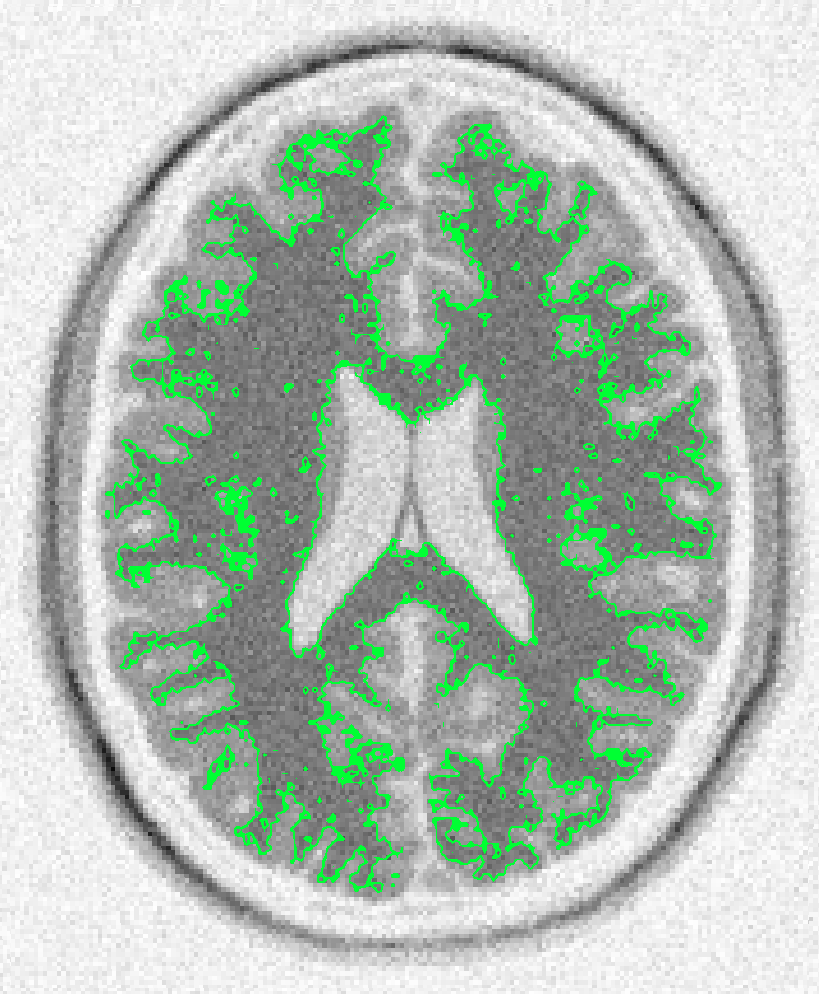
\includegraphics[width=3.05in]{figures/WithoutCurvature.png}
}
\subfigure[the same segmentation as above, using the same parameters, but under the influence of the curvature term]{
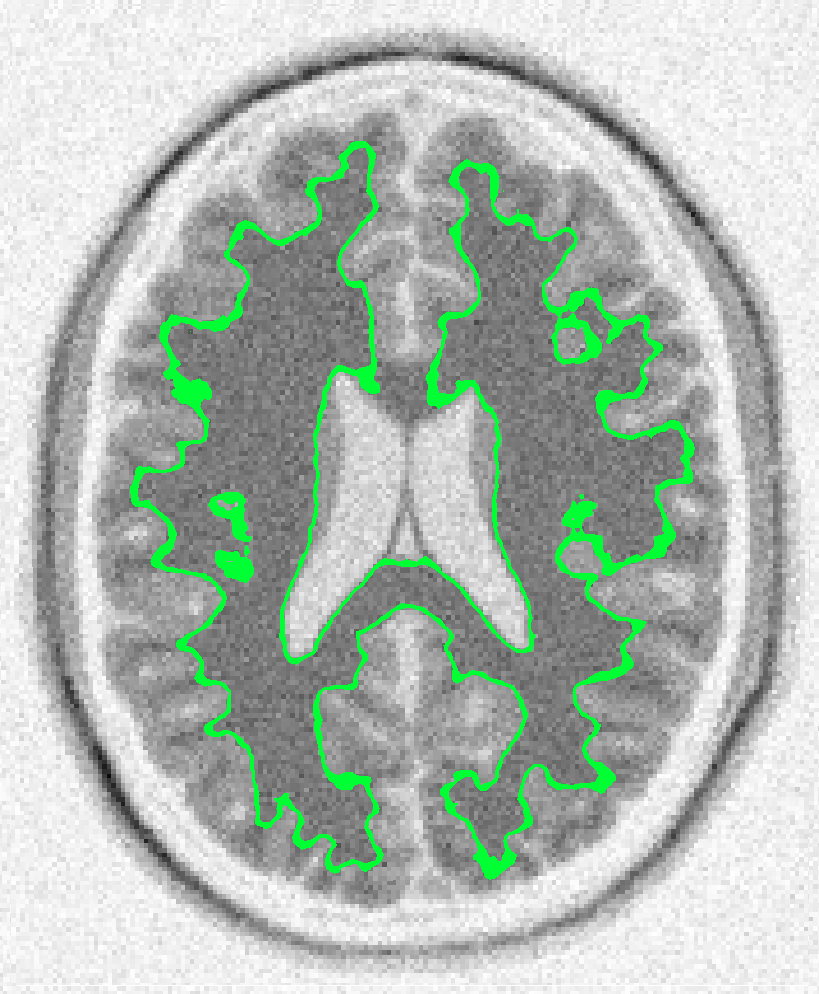
\includegraphics[width=3.05in]{figures/WithCurvature.png}
}
\caption{The effect of the curvature term in my speed function.}
\label{fig:curvatureeffect}
\end{figure}
%*******************************************************************************

As proposed by Lefohn et al.~\cite{Lefohn-2003-MICCAI,Lefohn-2003-Vis,Lefohn-2004}, I define the data term of my speed function $D \leftbracket \boldx \rightbracket = \varepsilon - \leftbracket \leftvbracket \ix \rightvbracket - T \rightbracket $ to be a function of the image intensity $\ix$, the user-specified target intensity $T$ that will encourage maximal surface growth, and a user-specified intensity window parameter $\varepsilon $ within which the level set surface is encouraged to grow. If $\ix$ is between $T-\varepsilon $ and $T+\varepsilon $, then $D \leftbracket \boldx \rightbracket $ will encourage surface growth, otherwise $D \leftbracket \boldx \rightbracket $ will encourage surface contraction. I define the curvature term of my speed function as $ C \leftbracket \boldx , t \rightbracket = \curvatureterm $, where $ \curvatureterm $ is the local mean surface curvature of the level set field from the previous iteration.

I define my speed function as $ F \leftbracket \boldx , t \rightbracket = \alpha C \leftbracket \boldx , t \rightbracket + \leftbracket 1 - \alpha \rightbracket D \leftbracket \boldx \rightbracket $ where $\alpha \in \leftsbracket 0 , 1 \rightsbracket $ is a user-specified blending term that controls the relative influence of the curvature and data terms on the behavior of my speed function. Figure \ref{fig:curvatureeffect} shows the effect of adjusting the relative influence of the curvature and data terms. For a detailed account of how this speed function can be implemented efficiently, I refer the reader to Lefohn et al.~\cite{Lefohn-2004}.

Intuitively speaking, I implicitly define my level set surface as the zero-level isosurface of a scalar field $\phi$. I implicitly evolve my level set surface by updating the scalar field $\phi$. Formally speaking, for the scalar field $ \phixt : \mathfrak{R}^4 \mapsto \mathfrak{R} $, I define my level set surface as $ \leftcbracket \boldx \mid \phixt = 0 \rightcbracket$. I express the level set field update equation as follows,
\begin{equation}
    \phixt = \phixtmdt + \Delta t F \leftbracket \boldx , t \rightbracket \leftvbracket \nabla \phixtmdt \label{eq:levelseteq}
\rightvbracket
\end{equation}
Two distinct algorithms for efficiently solving Equation~\ref{eq:levelseteq} are directly relevant to my work: the GPU narrow band algorithm~\cite{Lefohn-2003-MICCAI,Lefohn-2003-Vis,Cates-2004,Lefohn-2004,Jeong-2009} and the sparse field algorithm~\cite{Whitaker-1998,Peng-1999}.


%-------------------------------------------------------------------------
\subsection{The GPU Narrow Band Algorithm}

The narrow band algorithm~\cite{Adalsteinsson-1995} only computes level set field updates inside a small region (i.e. a narrow band) of elements around the implicitly defined level set surface. This algorithm has been successfully ported to the GPU~\cite{Lefohn-2003-MICCAI,Lefohn-2003-Vis,Cates-2004,Lefohn-2004,Jeong-2009} by using various virtual memory paging schemes to map the irregular and dynamic narrow band onto a physically contiguous domain better suited for GPU computation. These virtual memory paging schemes partition the level set field into tiles and map each active tile (i.e. each tile containing elements in the narrow band) to a contiguous physical block of GPU memory. GPU narrow band algorithms only perform level set computations on active tiles. This significantly improves performance and saves a large amount of GPU memory because inactive virtual tiles do not need to be stored on the GPU. In turn, this allows for images larger than the size of available GPU memory to be segmented.

Until very recently, GPU narrow band algorithms~\cite{Lefohn-2003-MICCAI,Lefohn-2003-Vis,Cates-2004,Lefohn-2004} have maintained the narrow band by using parallel data reduction techniques on the GPU in cooperation with the CPU. The GPU generates a down-sampled memory image of active tiles which is subsequently downloaded by the CPU at the end of each iteration. The CPU is responsible for traversing the down-sampled image, determining the narrow band for the next iteration, and communicating this result back to the GPU. Since the CPU must sequentially traverse the down-sampled image when updating the narrow band, these algorithms have $O(n)$ work-complexity~\cite{Atallah-1998} and $O(n)$ step-complexity~\cite{Nyland-2000} where $n$ is the size of the active computational domain. Moreover since the CPU work for each iteration cannot begin until the GPU work is finished and vice versa, these algorithms are limited by the communication latency between the GPU and CPU.

Developed in parallel with my own work, the GPU narrow band algorithm very recently described by Jeong et al.~\cite{Jeong-2009} avoids the communication latency inherent in previous GPU narrow band algorithms by traversing the domain of active tiles in parallel on the GPU. When a thread determines that a new tile should become part of the narrow band, the thread appends that tile to a list of active tiles stored in GPU memory. Since many threads are potentially appending to this list in parallel, Jeong et al.\ use GPU atomic memory operations to serialize access to the list. Therefore this system also has $O(n)$ work-complexity and $O(n)$ step-complexity.

%-------------------------------------------------------------------------
\subsection{The Sparse Field Algorithm}

In contrast to the GPU narrow band algorithm, the sparse field algorithm~\cite{Whitaker-1998,Peng-1999} incrementally updates a linked list of active elements on the CPU during each iteration. Therefore this algorithm's work-complexity is $O(n)$. The sparse field algorithm also reduces its total amount of work by a constant factor by tracking the active computational domain at the granularity of individual elements instead of tiles. Historically the sparse field algorithm has been poorly suited to parallel implementation due to its reliance on linked lists. Aside from the literature arising from the research in this thesis (see Appendix \ref{app:hpg}), no parallel implementation of the sparse field algorithm exists in the literature.

GPU narrow band systems~\cite{Lefohn-2003-MICCAI,Lefohn-2003-Vis,Cates-2004,Lefohn-2004,Jeong-2009} have historically outperformed optimized sequential sparse field systems~\cite{Ibanez-2005}. Nonetheless the GPU narrow band system I test in this thesis takes over 100 seconds to converge on the white and grey matter in a ${256}^3$ MRI of a human head on a state-of-the-art GPU. This limitation constrains clinical applications and motivates my work-efficient and step-efficient algorithm, which leverages ideas from both the GPU narrow band algorithm and the sparse field algorithm. I begin the presentation of my algorithm by describing my novel method for tracking the active computational domain.

